
\documentclass{beamer}

\usetheme{default}
\usepackage{tikz}
\usetikzlibrary{arrows,shapes.arrows,positioning,shapes}
\usepackage{graphicx}
\usepackage{hyperref}
\newcommand\red[1]{{\color{red}#1}}
\newcommand\bred[1]{{\color{red}\textbf{#1}}}
\newcommand\blue[1]{{\color{blue}#1}}
\newcommand\bblue[1]{{\color{blue}\textbf{#1}}}
\newcommand\green[1]{{\color{olive}#1}}
\newcommand\bgreen[1]{{\color{olive}\textbf{#1}}}
\newcommand\black[1]{{\color{black}#1}}
\newcommand\white[1]{{\color{white}#1}}
\newcommand\E{\text{E}}
\newcommand\V{\text{V}}
\renewcommand\P{\text{P}}
\def\vf{\vfill}
\newcommand{\indep}{{\bot\negthickspace\negthickspace\bot}}

\title{The Fragile Families Challenge:\\ \normalsize Predictability of family and child well-being in adolescence \vspace{-.2in}}

\author{Princeton Soc 300: Claims and Evidence}

%\institute[]
%{
%  Department of Sociology, Office of Population Research, \& \\Center for Research on Child Wellbeing, Princeton University}

\date{7 November 2018\\
\begin{flushleft}{\scriptsize
This research is supported by the Russell Sage Foundation.  We are grateful to the members of the Board of Advisors of the Fragile Families Challenge: Jeanne Brooks-Gunn, Kathryn J. Edin, Barbara E. Engelhardt, Irwin Garfinkel, Moritz Hardt, Dean Knox, Nicholas Lemann, Karen Levy, Sara McLanahan, Arvind Narayanan, Timothy J. Nelson, Matthew Salganik, \& Duncan Watts.  Source for these slides: \textcolor{blue}{\textcolor{blue}{\href{http://github.com/fragilefamilieschallenge}{www.github.com/fragilefamilieschallenge}}}. \includegraphics[width=0.05\textwidth]{figures/cc.png}}
\end{flushleft}
}

%\pgfdeclareimage[height=1cm]{university-logo}{ff_logo.jpg}
%\logo{\pgfuseimage{university-logo}}

%%%%%%%%%%%%%%%%%%%%%%%%%%%%%%
\begin{document}

\begin{frame}
  \titlepage
\end{frame}

%%%%%%%%%%%%%%%%%%%%%%%%%%
\begin{frame}

\begin{center}
\includegraphics[width=0.8\textwidth]{figures/wikipedia_logo}
\end{center}

\end{frame}
%%%%%%%%%%%%%%%%%%%%%%%%%%%
\begin{frame}

\begin{center}
\includegraphics[width=\textwidth]{figures/lander_initial_2001_title}
\end{center}

\vf
{\tiny \url{http://dx.doi.org/10.1038/35057062}}

\end{frame}
%%%%%%%%%%%%%%%%%%%%%%%%%%
\begin{frame}

\begin{center}
\includegraphics[height=\textheight]{figures/lander_initial_2001_authors}
\end{center}

\end{frame}
%%%%%%%%%%%%%%%%%%%%%%%%%%
\begin{frame}

\begin{center}
\includegraphics[width=\textwidth]{figures/aad_combined_2015_title}
\end{center}

\vfill
{\tiny \url{https://doi.org/10.1103/PhysRevLett.114.191803}}

\end{frame}
%%%%%%%%%%%%%%%%%%%%%%%%%%
\begin{frame}

\begin{center}
\only<1>{\includegraphics[height=\textheight]{figures/aad_combined_2015_authors_01}}
\only<2>{\includegraphics[height=\textheight]{figures/aad_combined_2015_authors_02}}
\only<3>{\includegraphics[height=\textheight]{figures/aad_combined_2015_authors_03}}
\only<4>{\includegraphics[height=\textheight]{figures/aad_combined_2015_authors_04}}
\only<5>{\includegraphics[height=\textheight]{figures/aad_combined_2015_authors_05}}
\only<6>{\includegraphics[height=\textheight]{figures/aad_combined_2015_authors_06}}
\only<7>{\includegraphics[height=\textheight]{figures/aad_combined_2015_authors_07}}
\only<8>{\includegraphics[height=\textheight]{figures/aad_combined_2015_authors_08}}
\only<9>{\includegraphics[height=\textheight]{figures/aad_combined_2015_authors_09}}
\only<10>{\includegraphics[height=\textheight]{figures/aad_combined_2015_authors_10}}
\only<11>{\includegraphics[height=\textheight]{figures/aad_combined_2015_authors_11}}
\only<12>{\includegraphics[height=\textheight]{figures/aad_combined_2015_authors_12}}
\only<13>{\includegraphics[height=\textheight]{figures/aad_combined_2015_authors_13}}
\only<14>{\includegraphics[height=\textheight]{figures/aad_combined_2015_authors_14}}
\only<15>{\includegraphics[height=\textheight]{figures/aad_combined_2015_authors_15}}
\only<16>{\includegraphics[height=\textheight]{figures/aad_combined_2015_authors_16}}
\end{center}

\end{frame}
%%%%%%%%%%%%%%%%%%%%%%%%%

\begin{frame}
\onslide<2-3>{Can we harness the power of \bblue{mass collaboration} in social science?}
\vskip .5cm
\onslide<3-3>{\bgreen{Key:} Ask a very specific question}
\end{frame}

\begin{frame}
\centering
\begin{tikzpicture}[x = .5\textwidth, y = .5\textheight]
\node at (0,.9) {\Large \blue{The Fragile Families Challenge}};
\onslide<1-2>{\node at (0,.75) {\large \blue{Predictability of family and child well-being in adolescence}};}
\onslide<3-3>{
	\node at (0,.75) {\large \bgreen{\underline{Predictability}} \blue{of family and child well-being in adolescence}};
	%\draw[->, line width = 2pt, olive] (-.95, .97) -- (-.8, .85);
	\draw[->, line width = 2pt, olive] (-.75, .95) -- (-.75, .82);
}
\node[align = center, font = \small] at (0, .5) {Claims and Evidence};
\node[align = center, font = \small] at (0, .25) {Princeton University};
\node[align = center, font = \small] at (0, 0) {7 November 2018};
\onslide<2-2>{
	\draw[->, line width = 3pt, olive] (.9, 0) -- (.7, -.2);
	\draw[line width = 2pt, olive, rounded corners] (-1.05,-.75) rectangle (1.05,-.25);
}
\node[align = center, font = \scriptsize] at (0, -.5) {\begin{minipage}{\textwidth}This research is supported by the Russell Sage Foundation.  We are grateful to the members of the Board of Advisors of the Fragile Families Challenge: Jeanne Brooks-Gunn, Kathryn J. Edin, Barbara E. Engelhardt, Irwin Garfinkel, Moritz Hardt, Dean Knox, Nicholas Lemann, Karen Levy, Sara McLanahan, Arvind Narayanan, Timothy J. Nelson, Matthew Salganik, \& Duncan Watts.  Source for these slides: \textcolor{blue}{\textcolor{blue}{\href{http://github.com/fragilefamilieschallenge}{www.github.com/fragilefamilieschallenge}}}. \includegraphics[width=0.05\textwidth]{figures/cc.png}\end{minipage}};
\end{tikzpicture}
\end{frame}

\begin{frame}
\centering
\begin{tikzpicture}[x = .5\textwidth, y = .5\textheight]
\node at (-1,-1) {};
\node at (1,1) {};
\node[font = \Large] at (0,.8) {Stratification can be framed as a \bgreen{predictive} question.};
\onslide<1-1>{
	\node[font = \Huge] at (0,.5) {$Y = \white{\underbrace{\black{\E\left(Y\mid \vec{X}\right)}}} + \epsilon$};
}
\onslide<8->{
	\node[font = \Huge] at (0,.5) {$Y = \underbrace{\E\left(Y\mid \vec{X}\right)} + \hspace{5pt}\epsilon$};
}
\onslide<2-3>{
	\node[font = \Huge] at (0,.5) {$\blue{Y} = \white{\underbrace{\black{\E\left(Y\mid \vec{X}\right)}}} + \epsilon$};
}
\onslide<4-5,7>{
	\node[font = \Huge] at (0,.5) {$Y = \blue{\underbrace{\E\left(Y\mid \vec{X}\right)}} + \epsilon$};
}
\onslide<6>{
	\node[font = \Huge] at (0,.5) {$Y = \blue{\underbrace{\beta_1X_1 + \beta_2X_2}} + \epsilon$};
}
\onslide<8-9>{
	\node[font = \Huge] at (0,.5) {$Y = \underbrace{\E\left(Y\mid \vec{X}\right)} +\blue{\hspace{5pt}\epsilon}$};
}
\onslide<2-3>{
	\node[font = \Large,blue,anchor=west] (attainment) at (-1,.2) {\bblue{Attainment}};
	\draw[->, line width = 1.5pt, blue] (-.6,0.4) -- (attainment);
}
\onslide<3-3>{
	\node[font = \Large,blue,anchor = west,align=left] (achievement) at (-1,0) {-- Academic\\\hspace{13pt}achievement};
}
\onslide<4-9>{
	\node[font = \Large,black,anchor = west,align=left] (achievement) at (-1,0) {-- Academic\\\hspace{13pt}achievement};
}
\onslide<4->{
	\node[font = \Large,anchor=west] (attainment) at (-1,.2) {\textbf{Attainment}};
	\draw[->, line width = 1.5pt] (-.6,0.4) -- (attainment);
}
\onslide<4-7>{
	\node[font = \Large,blue,anchor=north,align=center] (predictable) at (0.04,.15) {\bblue{Predictable}\\\bblue{component}};
	\draw[->, line width = 1.5pt, blue] (0.04, 0.25) -- (predictable);
}
\onslide<5-7>{
	\node[font = \Large,align=center,blue,anchor = west] (life_chances) at (-.2,-.2) {-- Life chances};
}
\onslide<8-9>{
	\node[font = \Large,align=center,anchor = west] (life_chances) at (-.2,-.2) {-- Life chances};
}
\onslide<8->{
	\node[font = \Large,anchor=north,align=center] (predictable) at (0.04,.15) {\textbf{Predictable}\\\textbf{component}};
	\draw[->, line width = 1.5pt] (0.04, 0.25) -- (predictable);
}
\onslide<8-9>{
	\node[font = \Large,align=center,blue] (unpredictable) at (.7,.1) {\bblue{Unpredictable}\\\bblue{component}};
	\draw[->, line width = 1.5pt, blue] (.63,0.4) -- (unpredictable);
}
\onslide<9-9>{
	\node[font = \Large,align=center,blue,anchor = west] (mobility) at (.45,-.1) {-- Mobility};
	\node[font = \Large,align=center,blue,anchor = west] (fluidity) at (.45,-.25) {-- Opportunity};
}
\onslide<10->{
	\node[font = \Large,align=center] (unpredictable) at (.7,.1) {\textbf{Unpredictable}\\\textbf{component}};
	\draw[->, line width = 1.5pt] (0.63,0.4) -- (unpredictable);
}
\onslide<10->{
	\node[font = \Large,anchor = west] at (-1.05,-.25) {\bblue{Puzzle}: Theories focus on the predictable component};
}
\onslide<11->{
	\node[font = \Large,anchor = west] at (-1.05,-.4) {but empirically the unpredictable component dominates.};
}
\onslide<12->{
	\node[font = \Large,anchor = west] at (-1.05, -.55) {\bblue{Candidate explanation:} Modeling errors};
	\node[font = \Large] at (0, -.75) {$\hat\E\left(Y\mid \vec{X}\right) \neq \E\left(Y\mid \vec{X}\right)$.};
}
\end{tikzpicture}
\end{frame}

\begin{frame}
\Large
\bgreen{Modeling errors}\onslide<4->{ can be minimized by \\\bblue{machine learning}.} \\
\begin{center}
\begin{tikzpicture}[x = .8\textwidth, y = .5\textheight]
\pause
\node at (-.95,-.1) {$Y$};
\node (y) at (-.9,-.1) {$\bullet$};
\node at (0,0.15) {$\hat{\E}_\text{OLS}\left(Y\mid \vec{X}\right)$};
\node (ols) at (0,0) {$\bullet$};
\draw[thick] (ols) -- (y);
\pause
\node at (-.75,.3) {$\E\left(Y\mid \vec{X}\right)$};
\node (e) at (-.75,.15) {$\bullet$};
\draw[thick] (e) -- (y);
\pause \pause
\node at (-.4,.35) {$\hat{\E}_\text{ML}\left(Y\mid \vec{X}\right)$};
\node (ml) at (-.4,.2) {$\bullet$};
\draw[thick] (ml) -- (y);
\end{tikzpicture}
\end{center}
\onslide<6->{
	\bgreen{How much does predictability improve} when we\\
	utilize this \bblue{untapped modeling potential}?
}
\end{frame}



%% SLIDES FROM PRIOR PRESENTATIONS HERE %%

\begin{frame}

\begin{center}
\includegraphics[width=\textwidth]{figures/ff_logo}
\end{center}

\begin{itemize}
\item Birth cohort panel study
\item $\approx$ 5,000 children born in 20 U.S. cities
\item Followed from birth through age 15
\end{itemize}

\end{frame}
%%%%%%%%%%%%%%%%%%%%%%%%%
\begin{frame}

\begin{center}
\only<1>{\includegraphics[height=0.8\textheight]{figures/ff_design_public_b9}}
\only<2>{\includegraphics[height=0.8\textheight]{figures/ff_design_public_b9_15}}
\end{center}

\end{frame}
%%%%%%%%%%%%%%%%%%%%%%%%%
%\begin{frame}

%\begin{center}
%\includegraphics[width=\textwidth]<1>{figures/ff_design_matrix_ml}
%\includegraphics[width=\textwidth]<2>{figures/ffc_design_matrix_ml}
%\end{center}

%\end{frame}
%%%%%%%%%%%%%%%%%%%%%%%%%
\begin{frame}

Six age 15 outcomes:
\begin{itemize}
\item GPA
\item Material Hardship
\item Grit
\item Evicted
\item Job training
\item Job loss
\end{itemize}

\end{frame}
%%%%%%%%%%%%%%%%%%%%%%%%%
\begin{frame}

441 registered participants
\begin{itemize}
\item social scientists and data scientists
\item undergraduates, grad students, and professionals
\item many working in teams
\end{itemize}

\end{frame}
%%%%%%%%%%%%%%%%%%%%%%%%%%%
\begin{frame}

\begin{center}
How did they do?
\end{center}

\end{frame}
%%%%%%%%%%%%%%%%%%%%%%%%%%%
\begin{frame}

Before I show you, let's vote . . .

\end{frame}
%%%%%%%%%%%%%%%%%%%%%%%%%%%
\begin{frame}

\centering
\includegraphics[width=\textwidth]{figures/RSquared_all_ASA.pdf}

\end{frame}
%%%%%%%%%%%%%%%%%%%%%%%%%%%
\begin{frame}

\centering
\includegraphics[width=\textwidth]{figures/RSquared_all_ASA_01.pdf}

\end{frame}
%%%%%%%%%%%%%%%%%%%%%%%%%%%
\begin{frame}

\centering
\includegraphics[width=\textwidth]{figures/RSquared_all_ASA_01_benchmark.pdf}

\end{frame}
%%%%%%%%%%%%%%%%%%%%%%%%%%%

\begin{frame}{What we learned}
\large
Hundreds of teams tried many modeling strategies. \\
Predictions were poor. \\
That's the best we could do. \pause
\begin{center}
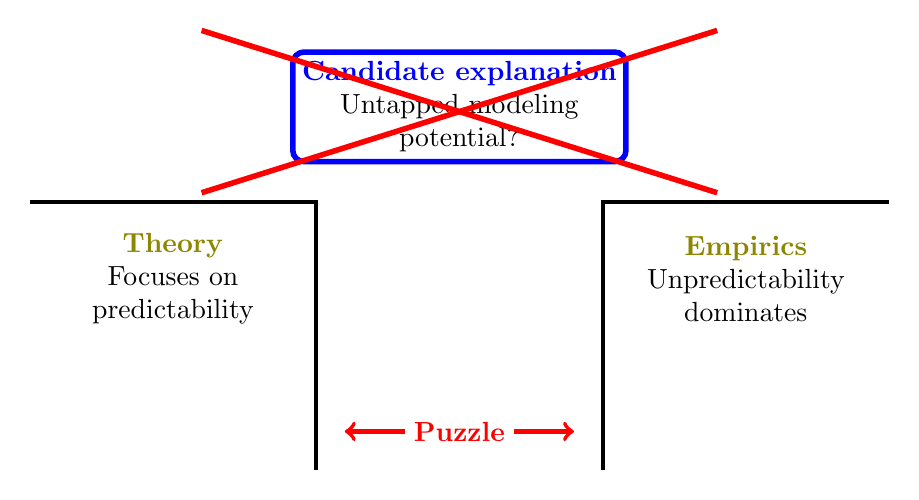
\begin{tikzpicture}[x = .3\textwidth, y = .2\textwidth]
\onslide<2-5>{
\node[align = center] at (-1, -1) {\bgreen{Theory}\\Focuses on\\predictability};
\draw[line width = 1.5pt] (-1.5, -.6) -- (-.5, -.6) -- (-.5, -2);
\draw[line width = 1.5pt] (1.5, -.6) -- (.5, -.6) -- (.5, -2);
\node[align = center] at (1, -1) {\bgreen{Empirics}\\Unpredictability\\dominates};
\draw[<->, line width = 1.5pt, red] (-.4, -1.8) -- (.4, -1.8);
\node[align = center, fill = white] at (0, -1.8) {\bred{Puzzle}};
}
\onslide<3-4>{
\node[align = center, draw = blue, line width = 2pt, rounded corners] at (0, -.1) {\bblue{Candidate explanation}\\Untapped modeling\\potential?};
}
\onslide<4-4>{
\draw[line width = 2pt, red] (-.9, -.55) -- (.9, .3);
\draw[line width = 2pt, red] (-.9, .3) -- (.9, -.55);
}
\end{tikzpicture}
\end{center}
\end{frame}

%%%%%%%%%%%%%%%%%%%%%%%%%%%

\end{document}

%% OLD %%

